\section{Solución propuesta}

Las reservas de habitaciones pueden ser un problema, dado que hay que tener en cuenta las fechas disponibles y la coordinación entre el cliente y la posada. Por eso, lo que nosotros proponemos es una aplicación web que resulte atractiva, llamativa y que provea a los clientes una forma sencilla y cómoda de reservar, sin pasar por consultas por mail o Whatsapp. En lugar de eso, el que esté interesado en poder estanciarse en la posada puede encontrar en el calendario las fechas en las que desea hospedarse y la página realiza la consulta. El cliente luego confirma la reserva y en el caso que se quiera revertir la reserva lo podrá hacer introduciendo sus datos y un código que se le es otorgado para lograr mas seguridad tanto para el cliente como para la misma reserva de la página.

La estructura del proyecto consta de una API (Application Program Interface) y de un servidor web, ambas son aplicaciones separadas que se complementan para el buen funcionamiento de la página. En la figura \ref{fig:Est} se puede observar como la parte del servidor web contiene toda el frente de la página, capaz de generar interactividad y comunicación con el cliente, 



\begin{figure}
    \centering
    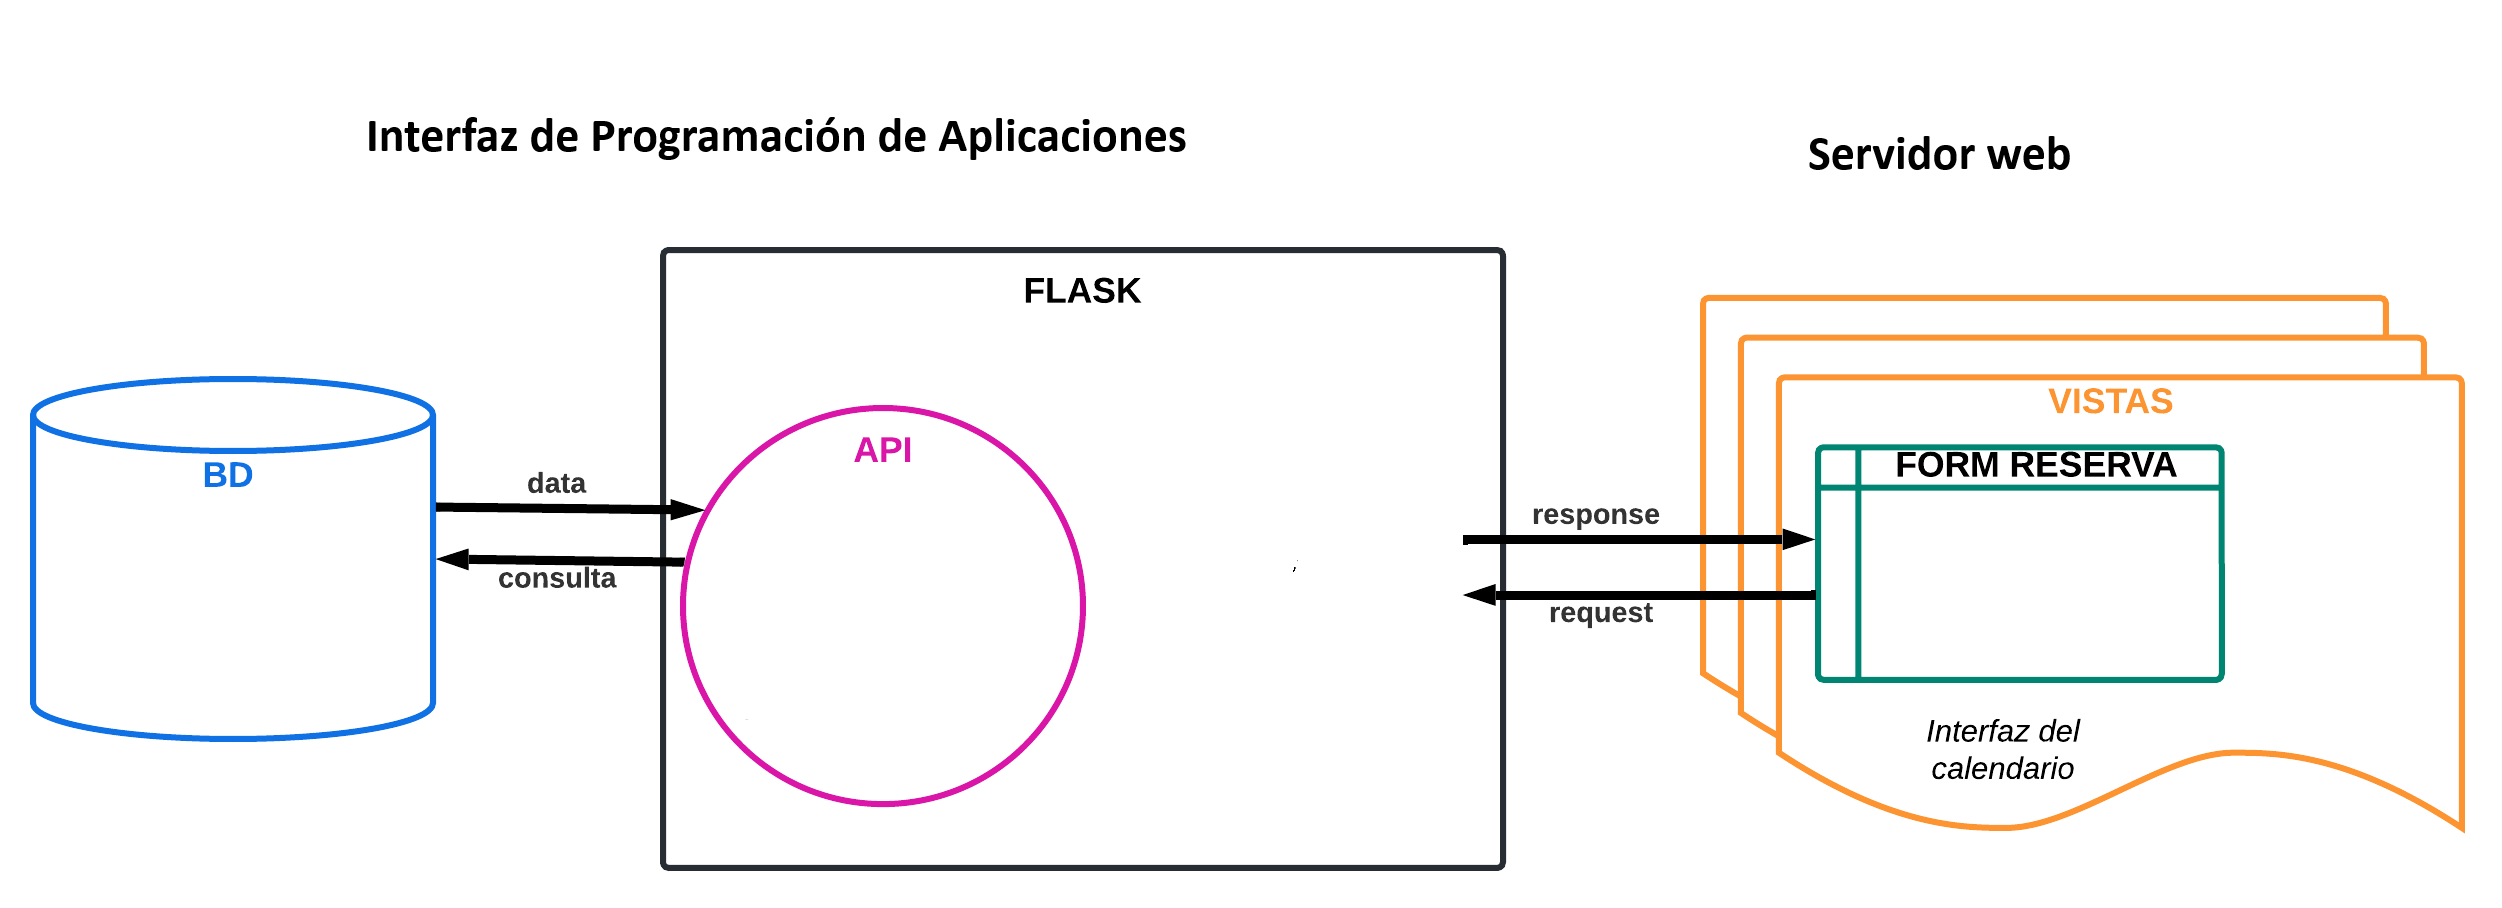
\includegraphics[width=1\linewidth]{images/Estructura_de_pagina.png}
    \caption{Estructura del proyecto}
    \label{fig:Est}
\end{figure}